\subsection{Overlaping to Hide Latency}



\begin{figure}[h!]
  \centering
    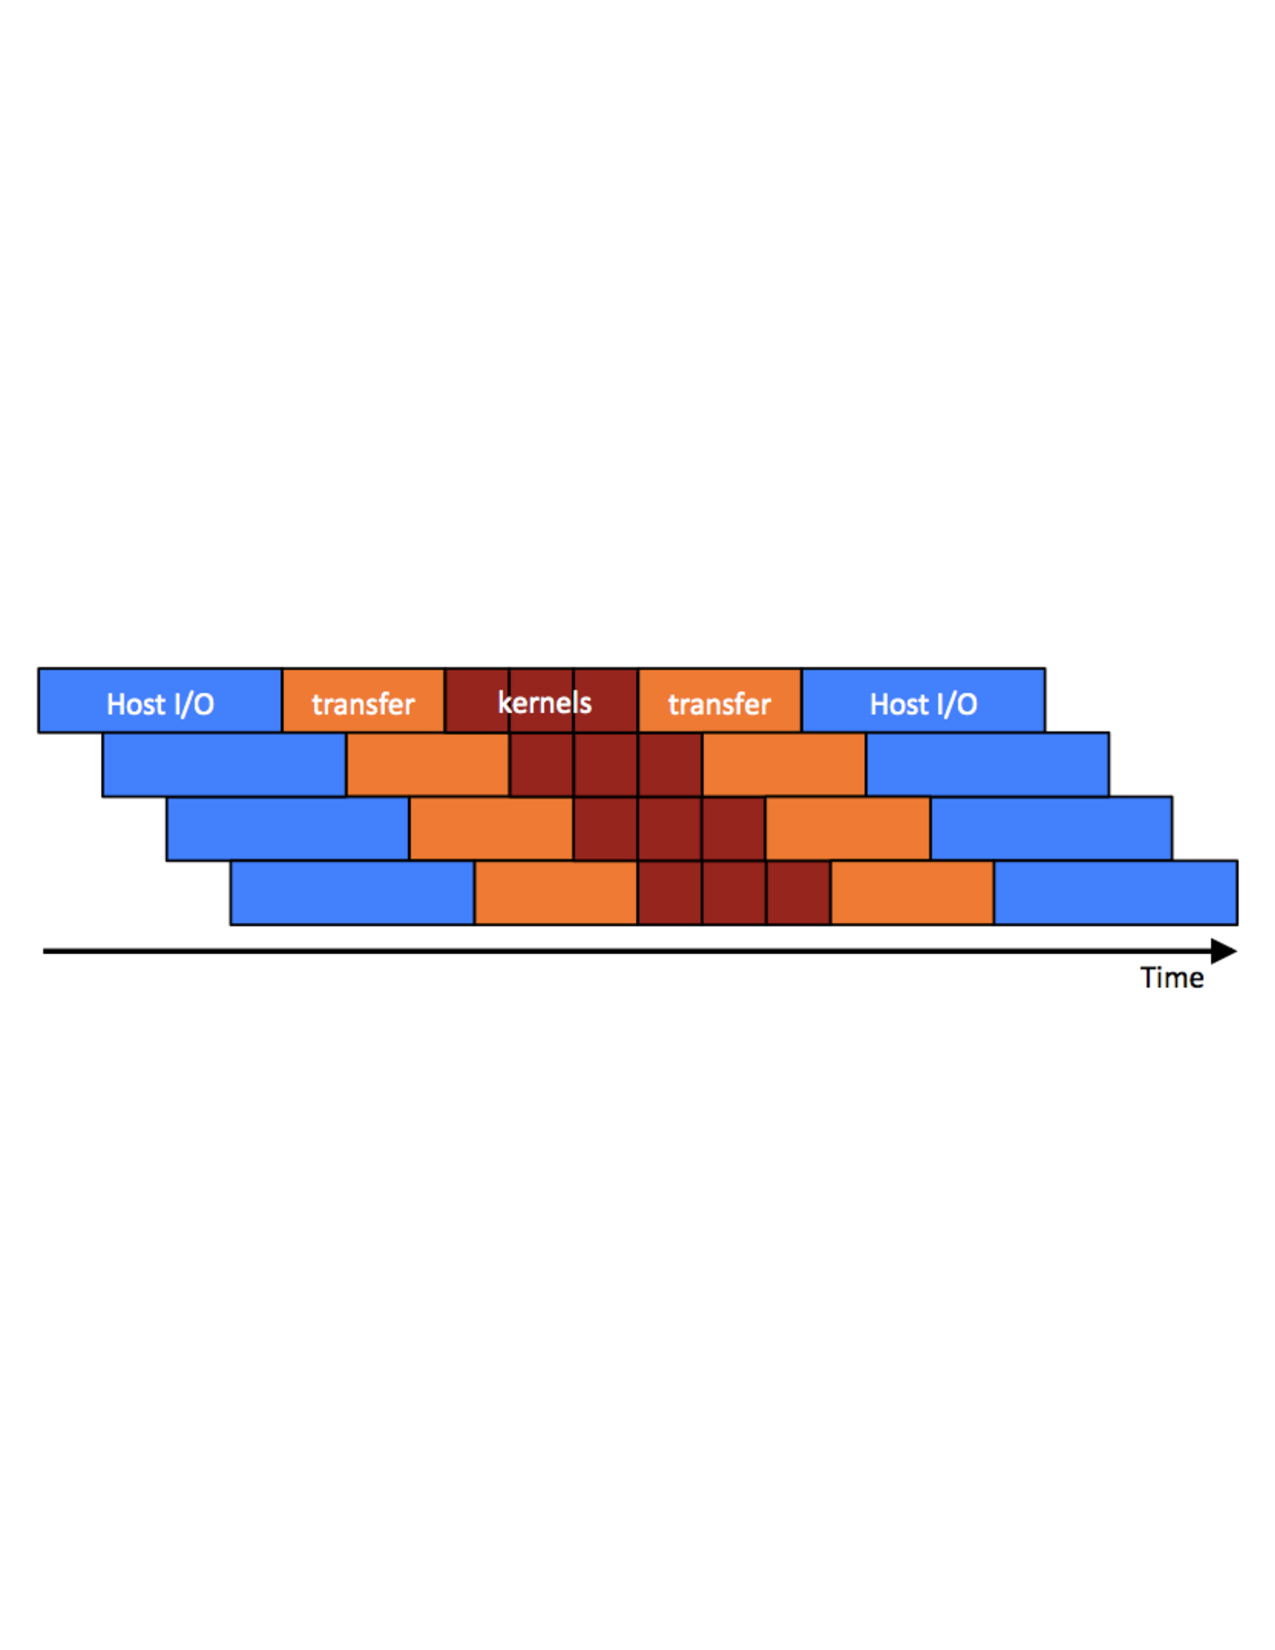
\includegraphics[width=0.5\textwidth]{fig/ordered.pdf}
  \caption{A representation of simple overlap of host I/O, host-to-device data
           transfer, and kernel execution. In this example, there are no
           dependencies between kernels and data so management is relateively
           simple.}
\end{figure}

\begin{figure}[h!]
  \centering
    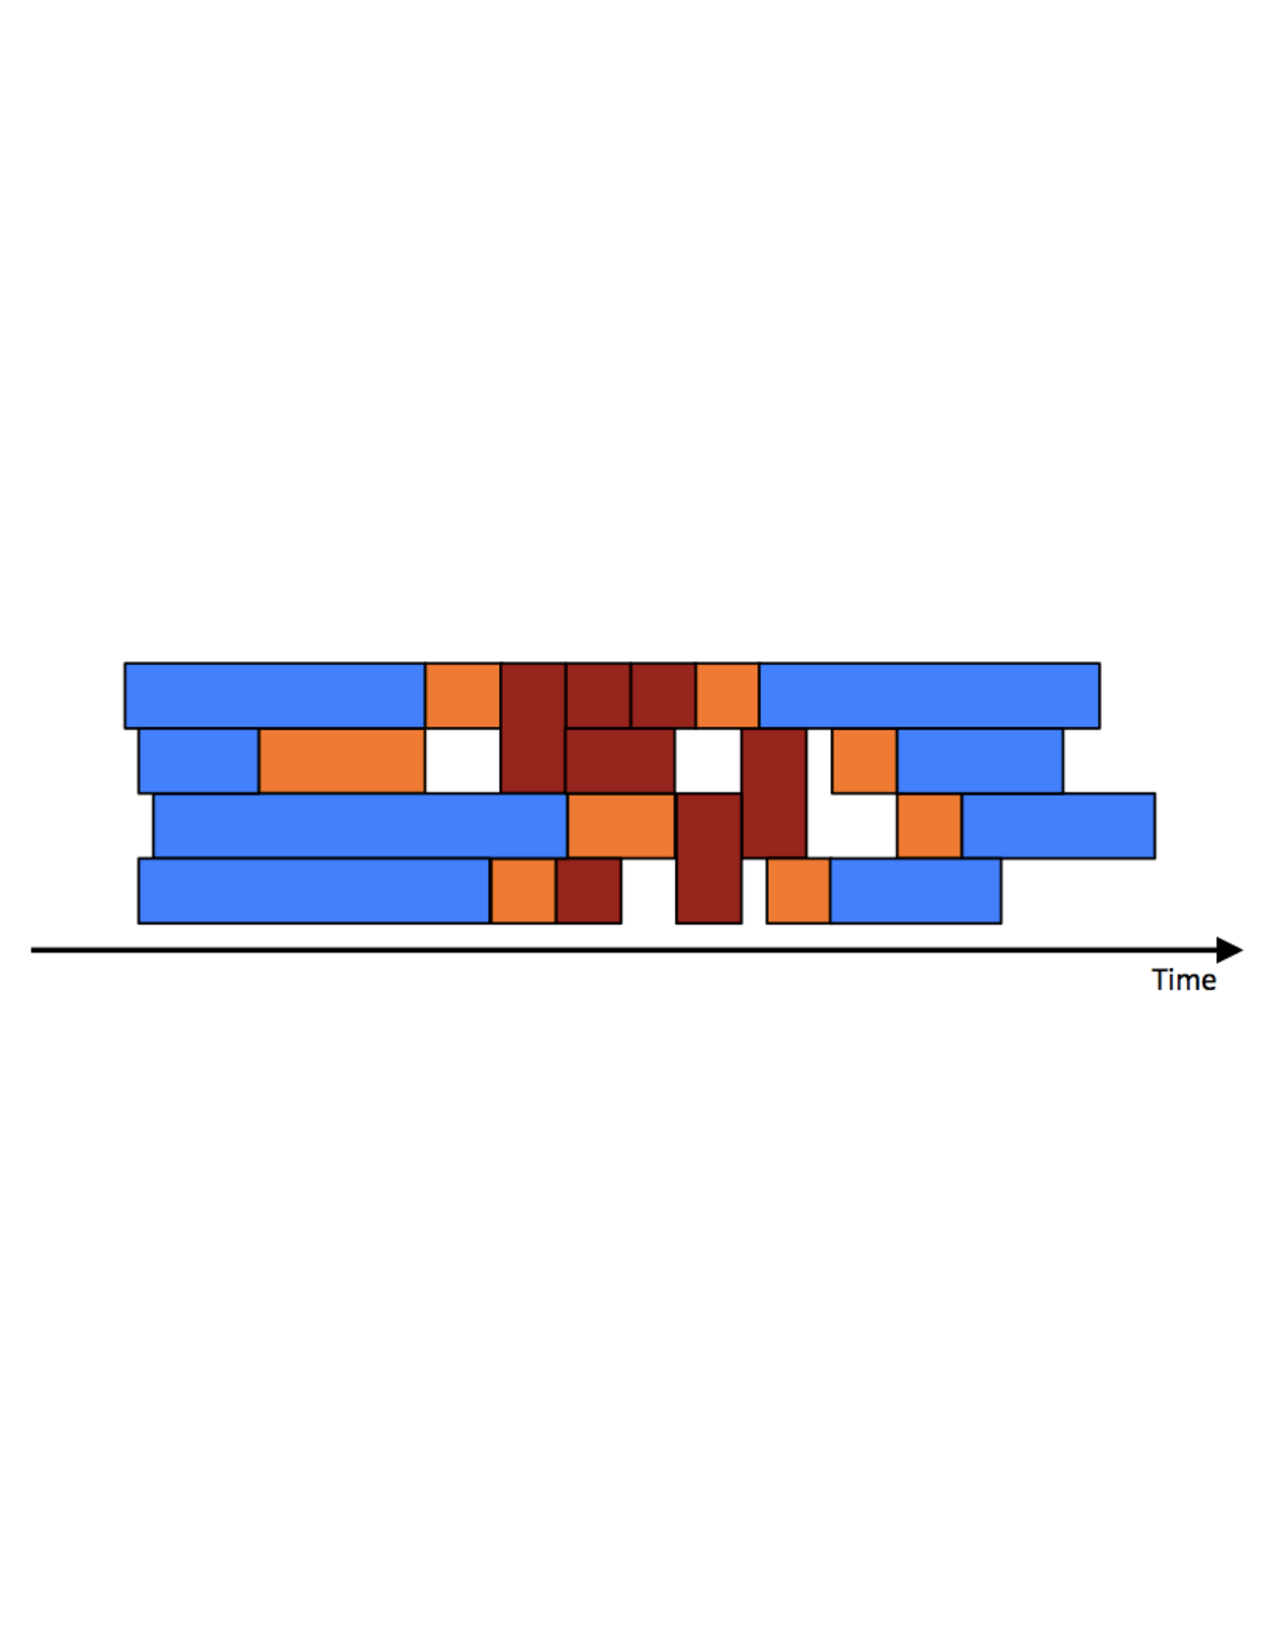
\includegraphics[width=0.5\textwidth]{fig/unordered.pdf}
  \caption{A more complicated oververlap of host I/O, host-to-device data
           transfer, and kernel execution. Arbitrary data-dependence between
           kernels and transfers places too large a burden on the programmer
           to manage properly.}

\end{figure}

